\documentclass[aspectratio=169,xcolor=dvipsnames]{beamer}
\usetheme{Berlin}

\usepackage[english]{babel}
\usepackage{hyperref}
\usepackage{graphicx}
\usepackage{booktabs}
\usepackage{amsmath}
\usepackage{amssymb}
\usepackage{lettrine}
\setbeamertemplate{caption}[numbered]
\usepackage[dvipsnames,svgnames,x11names]{xcolor}
\usepackage{xurl}
\usepackage{algorithm}
\usepackage{algorithmicx}
\usepackage{algpseudocode}
\usepackage{adjustbox}

\hypersetup{
    colorlinks=true,
    linkcolor=cyan,
    filecolor=blue,
    urlcolor=blue,
    citecolor=blue,
}

%----------------------------------------------------------------------------------------
%   CODE LISTINGS SETTINGS
%----------------------------------------------------------------------------------------
\usepackage{listings}
\definecolor{backcolour}{rgb}{0.97,0.97,0.99}
\definecolor{codegreen}{rgb}{0,0.6,0}

\lstdefinestyle{MATLABStyle}{
  language=Matlab,
  basicstyle=\ttfamily\scriptsize,
  keywordstyle=\color{blue}\bfseries,
  commentstyle=\color{codegreen},
  stringstyle=\color{violet},
  breaklines=true,
  numbers=left,
  numbersep=5pt,
  frame=lines,
  backgroundcolor=\color{backcolour}
}
\lstset{style=MATLABStyle}

%----------------------------------------------------------------------------------------
%   TITLE CONFIGURATION
%----------------------------------------------------------------------------------------
\title{Mathematical Modeling of Physical Systems}
\subtitle{Simulation of Systems and Processes}
\author{Prof. D.Sc. BARSEKH-ONJI Aboud}
\institute{
    Facultad de Ingenier\'ia \\
    Universidad An\'ahuac M\'exico
}
\date{\today}

%----------------------------------------------------------------------------------------
%   AUTO AGENDA AT EACH SECTION
%----------------------------------------------------------------------------------------
\AtBeginSection[]{
  \begin{frame}{Agenda}
    \tableofcontents[currentsection]
  \end{frame}
}

\begin{document}

\begin{frame}
    \titlepage
\end{frame}

\begin{frame}{Table of Contents}
    \tableofcontents
\end{frame}

%------------------------------------------------
\section{Introduction}
%------------------------------------------------

\subsection{What is Mathematical Modeling}
\begin{frame}{Introduction -- Mathematical Modeling}
    \begin{block}{Why we model physical systems}
        The task of mathematical modeling is an important step in the analysis and design of physical systems. In this conference, we will develop mathematical models for mechanical, electrical, hydraulic, and thermal systems. The mathematical models of systems are obtained by applying the fundamental physical laws that govern the nature of the components making these systems.
    \end{block}
\end{frame}

\subsection{Real Systems vs. Mathematical Modeling}
\begin{frame}{Real Systems vs. Mathematical Modeling}
    \begin{alertblock}{Idealization is unavoidable}
        Real systems are usually quite complex and exact analysis is often impossible. We shall make approximations and reduce the system components to idealized versions whose behaviors are similar to the real components.
    \end{alertblock}
\end{frame}

\subsection{Laplace Transformation \& Differential Equations}
\begin{frame}{Laplace Transformation \& Differential Equations}
    \begin{block}{From differential equations to transfer functions}
        The mathematical model of a system is one that consists of one or more differential equations that describe the dynamic behavior of the system. \textbf{The Laplace transformation is applied to the mathematical model and then the model is converted into an algebraic equation.} The properties and behavior of the system can then be represented as a block diagram, with the \textbf{transfer function} of each component describing the relationship between its input and output behavior.
    \end{block}
\end{frame}

%------------------------------------------------
\section{State-Space Modeling}
%------------------------------------------------

\subsection{What is a State-Space System?}
\begin{frame}{What is a State-Space System?}
    \begin{block}{Definition}
        State refers to the past, present, and future condition of the system from a mathematical cell. State could be defined as a set of state variables and state equations to model the dynamic system. All the state equations are first-order differential equations.
    \end{block}
\end{frame}

\subsection{State Variables and Equations}
\begin{frame}{State Variables and Equations}
    \begin{block}{State variables}
        It is defined as the minimal set of variables $[x_1(t), x_2(t), \dots, x_n(t)]$ such that knowledge of these variables at any time $t = 0$ and information on the input excitation subsequently applied are sufficient to determine the state of the system at time $t > t_0$.
    \end{block}
    \begin{alertblock}{Common confusion}
        One is likely to confuse state variables with output variables. Output variables can be measured, but state variables do not always satisfy this condition.
    \end{alertblock}
\end{frame}

\begin{frame}{State Equation and Output Equation}
    The variable $U(t)$ is controllable at all time instants $t > t_0$. The input $U(t)$ is taken from the input space. The output variable $Z(t)$ is observable at all time instants $t > t_0$, but there is no direct control on the output variables. $Z(t)$ is taken from the universe of output $Z$.

    \begin{block}{State equation}
        \begin{equation}
            \dot{X}(t) = A X(t) + B U(t)
        \end{equation}
    \end{block}

    \begin{block}{Output equation}
        \begin{equation}
            Z(t) = C X(t) + D U(t)
        \end{equation}
    \end{block}
\end{frame}

%------------------------------------------------
\section{Examples}
%------------------------------------------------

\subsection{Moving Car Simple Model}
\begin{frame}{Moving Car Simple Model}
    \begin{exampleblock}{Example 1}
        Please check this link: \href{https://la.mathworks.com/help/simulink/gs/create-a-simple-model.html}{\textbf{Moving car simple model}}
    \end{exampleblock}
    \begin{figure}
        \centering
        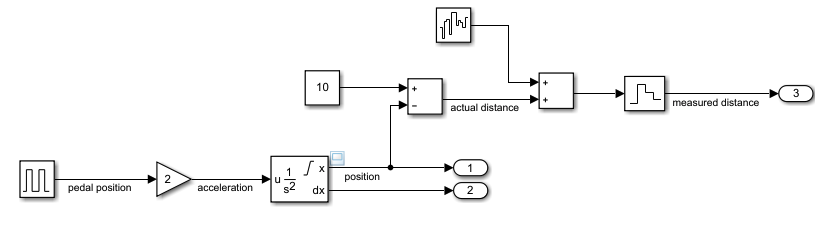
\includegraphics[width=0.8\textwidth,height=0.6\textheight,keepaspectratio]{figs/fig11.png}
        \caption{Moving car simple model}
        \label{fig:moving-car}
    \end{figure}
\end{frame}

\subsection{Simple Mechanical Translational System}
\begin{frame}{Simple Mechanical Translational System}
    \begin{figure}
        \centering
        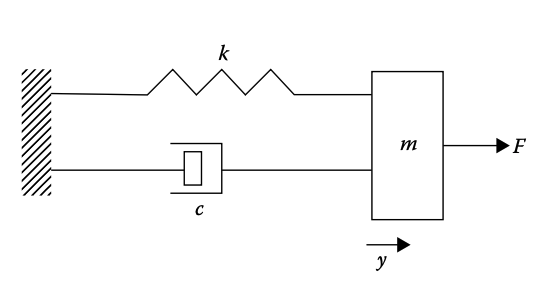
\includegraphics[width=0.55\textwidth,height=0.7\textheight,keepaspectratio]{figs/model2.png}
        \caption{Simple mechanical system}
        \label{fig:mech-system}
    \end{figure}
\end{frame}

\begin{frame}{Simple Mechanical Translational System -- Equations}
    \footnotesize
    \begin{block}{Derivation}
        \begin{equation}
            F - ky - b \frac{dy}{dt} = m \frac{d^2y}{dt^2}
        \end{equation}
        \begin{equation}
            F = m \frac{d^2y}{dt^2} + b \frac{dy}{dt} + ky
        \end{equation}
        \begin{equation}
            F(s) = ms^2Y(s) + bsY(s) + kY(s)
        \end{equation}
        \begin{equation}
            \frac{Y(s)}{F(s)} = \frac{1}{ms^2 + bs + k}
        \end{equation}
    \end{block}
\end{frame}

\subsection{Van Der Pol Equation}
\begin{frame}{Van Der Pol Equation}
    \begin{block}{Model}
        \begin{equation}
            \ddot{y} + \mu (y^2 - 1) \dot{y} + y = 0
        \end{equation}
        $\mu=1$, $X_{01}=1$, $X_{02}=-2$
    \end{block}
    \begin{figure}
        \centering
        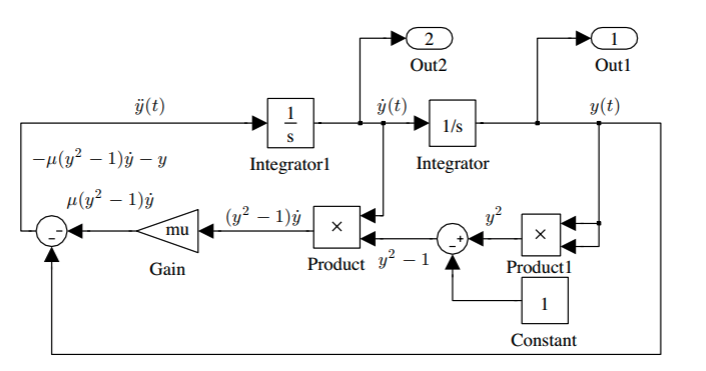
\includegraphics[width=0.5\textwidth,height=0.6\textheight,keepaspectratio]{figs/Van.png}
        \caption{Van Der Pol equation model}
        \label{fig:van-der-pol}
    \end{figure}
\end{frame}

%------------------------------------------------
\section{Activity}
%------------------------------------------------

\begin{frame}{Activity}
    \begin{figure}
        \centering
        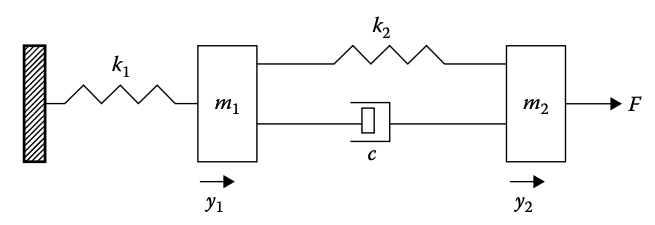
\includegraphics[width=0.7\textwidth,height=0.65\textheight,keepaspectratio]{figs/act.png}
        \caption{Mechanical system with two masses and two springs: $m_1=1$, $m_2=1.5$, $B=0.1$, $K_1=0.2$, $K_2=0.15$}
        \label{fig:activity}
    \end{figure}
\end{frame}

\end{document}
